\documentclass[../Thesis.tex]{subfiles}
 
\begin{document}
 
\section  {Preprocessing}
\subsection {Audio Decoding}

We are only going to work with two different audio formats: \texttt{.wav} (Waveform Audio File) and \texttt{.mp3} (MPEG-2 Audio Layer III). The wav files are used in training and evaluating the model, while the mp3 files are only used when received from the user, or to pass the resulting audio file back to the user.

To decode both formats, we are using \texttt{open} and \texttt{load} functions provided by Librosa. The mp3 can be open and transformed into a waveform. The wav files are already stored as a waveform, so we only need to open the file and extract it. After we are done processing the waveform, we have to encode and save it to file. Fot this we have the \texttt{write\_wav} and \texttt{sf.write} function.


\subsection {Data Preparation}

The DSD100 dataset must be acquired and added to the project. The dataset consists of 100 full lengths music tracks, and their isolated bass, vocals, drums and accompaniment, all saved under the \texttt{wav} file format. 50 songs are found in the \texttt{dev} folder, meaning there are meant for training, and another 50 are in the \texttt{test} folder, which is meant to use for evaluating. We are actually going to use both for training our model. This will improve it, but will make the tuning phase a little more difficult. To ensure the mixture is a perfect combination of the 2 sources, the mixture will be computed in our code, after the two different wavs are opened. A simple arithmetic mean of the two waveforms will do the trick.

The wavs need to be further translated to the equivalent spectrograms. This will be done using the \texttt{stft} method provided by Librosa. We will be more interested in the magnitude spectra. The phase spectra are not needed for the training phase. They will be used to reconstruct the audios after they are separated, but have no impact on the training of the network. Just another method \texttt{spec\_to\_batch} is required in order to transform the spectra to a batch that can be passed to our model. This method just reshapes and adds padding where needed.


\section {Model}
\subsection {Architecture}

Here we have an overview of the overall architecture for our neural network. As mentioned before, we have decided to use the LSTM variation of the RNN. The network will consist of an input layer, 3 hidden layers with LSTM cells, 2 fully connected (dense) layers and another 2 layers representing the time-frequency masking layer. We will discuss these layers in detail below.
The loss function defined by:  $\mathit{loss} = \mathit{mean}( {( \mathit{y}_{1\mathit{p}} – \mathit{y}_1 )}_{}^2 + {( \mathit{y}_{2\mathit{p}} – \mathit{y}_2 )}_{}^2)$ , 
where: $ \mathit{y}_{1\mathit{p}} $ – predicted source 1 magnitude tensor, $ \mathit{y}_{1} $ – source 1 magnitude tensor, $ \mathit{y}_{2\mathit{p}} $ – predicted source 2 magnitude tensor, $ \mathit{y}_{2} $ – source 2 magnitude tensor 

\begin{figure}[h]
\centering
\label {fig: data_flow}
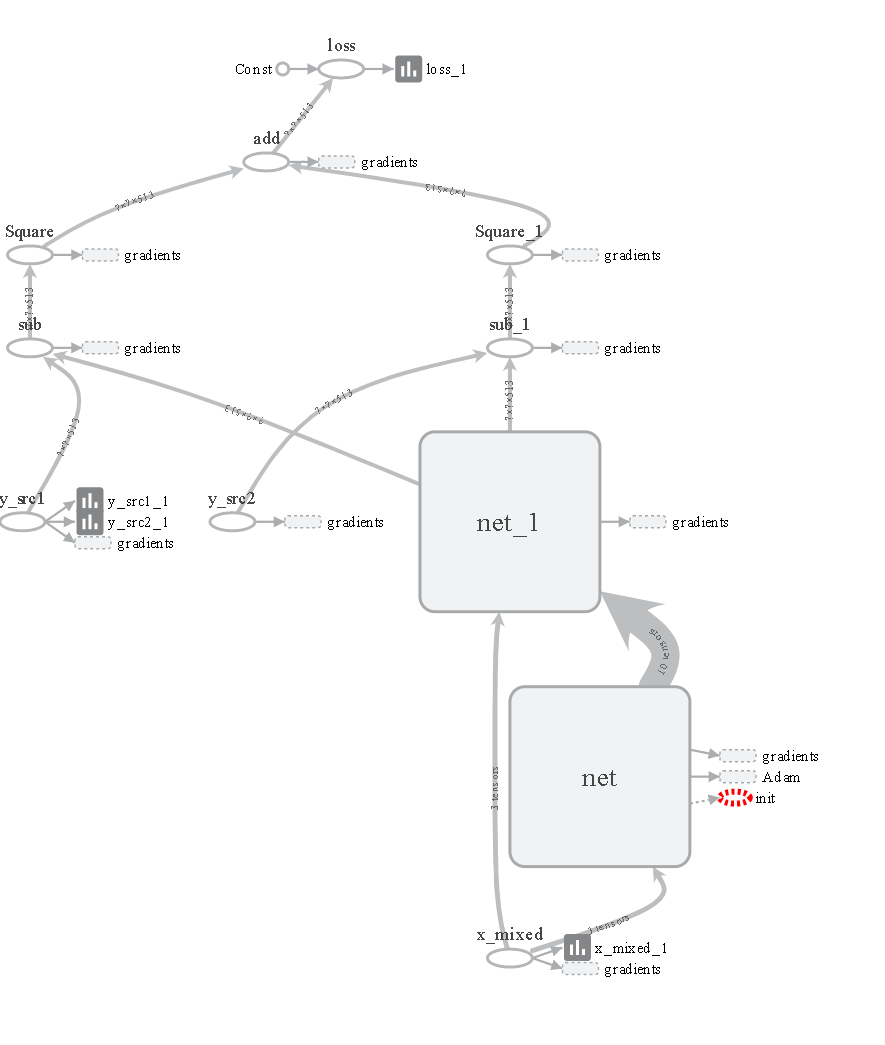
\includegraphics[width=0.5\textwidth]{data_flow.png}
\caption[width=0.5\textwidth]{visualization of the data flow in TensorBoard}
\end{figure}

\begin{figure}[h]
\centering
\label {fig: layers}
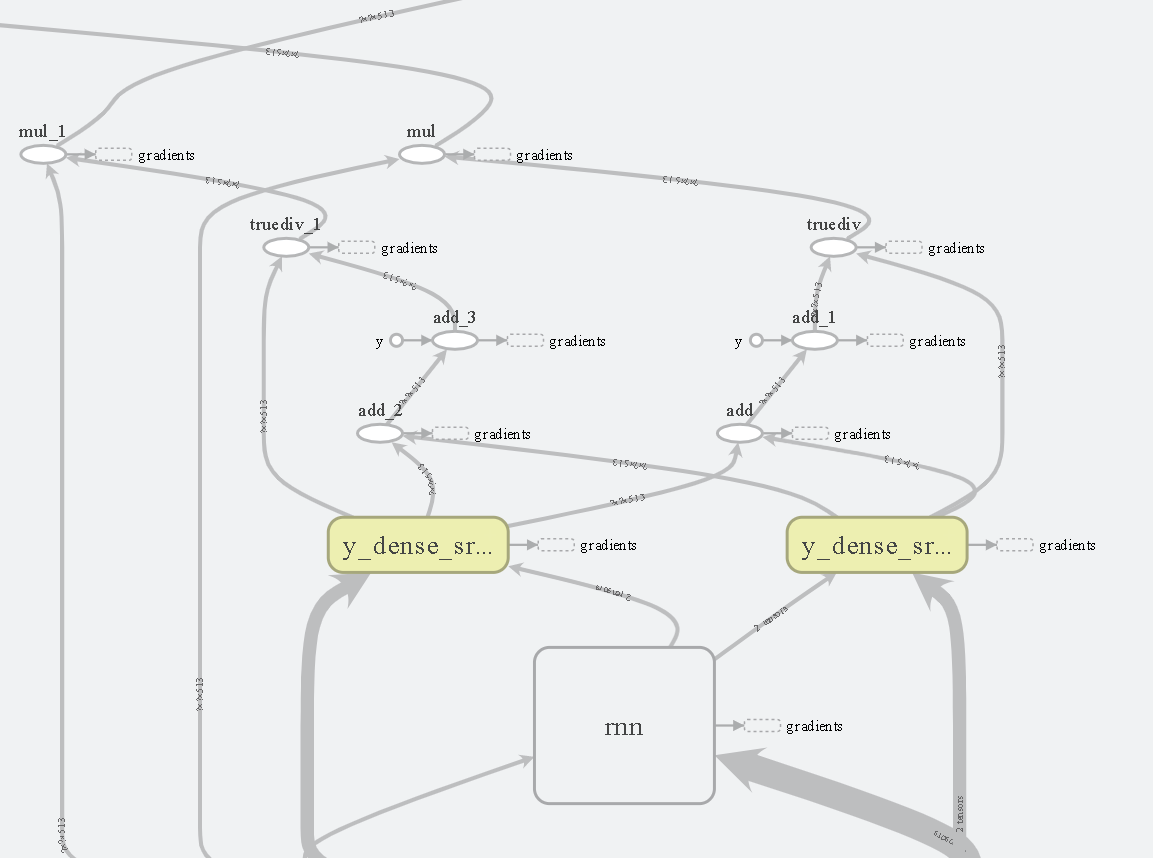
\includegraphics[width=0.5\textwidth]{layers.png}
\caption[width=0.5\textwidth]{LSTM, dense and masking layer viewed in TensorBoard}
\end{figure}

\subsection {Configuration}

Here we will have an overview over the configurable part, and what it represents. Looking at the more important hyperparameters we have: sample rate for the audio files, frame length of the spectrograms, learning rate, checkpoint step and number of seconds of the training audios (batch size). The sample rate is 44100, as the songs are also encoded at this value of Hertz. Frame length of the spectrograms is 1024, the default one using the Librosa package. Learning rate is not fixed. We might start with a 0.001 learning rate and decrease it at about 80\% training, so the model can better tune the features found. Checkpoints should be done as frequently as possible to make sure we aren’t losing progress. This parameter is dependent on the number of training iterations. The batch size is 8.192 seconds. I chose this exact number so we can draw a Mel spectrogram of size 512:512 from the batch if we ever want to visualize the data.

Other objects like session configuration or data path are available in a configuration file. 
We will only train the model to recognize drums and vocals from a mixture of the two. This should be a good start giving the limited time and data available. 


\subsection {Layers}
\subsubsection {Input Layer}

Input layer is composed by a tensor, containing floats, and representing a frame from the magnitude spectrum of the mixture. We create a placeholder for the tensor, using \texttt{tf.placeholder} and call it \texttt{x\_mixed}. We specify one of the dimensions’ size to be equal to half the length of a frame from our spectrogram. This layer is connected to the LSTM layer through edges with trainable weights.

\subsubsection {LSTM Cells}

A configurable number (default 3) of LSTM layers defined. To do this, an LSTM cell must be created for each layer. The size of those cells is hardcoded to 256.To create the LSTM cells we call \texttt{rnn\_cell.LSTM} and provide the mentioned size and to define the layers we use the method \texttt{rnn\_cell.MultiRNNCell} The RNN is created by calling \texttt{tf.nn.dynamic\_rnn}. The input layer will act as input and the LSTM layers defined will act as the core of this network. The output of this network will pass on to two fully connected layers.

\subsubsection {Dense Layer}

Two fully connected layers (one for each source) are formed right after the RNN. These layers will hopefully find patterns that identify each source. It’s important that these two layers are located right after the RNN in order to get information on past data as well.  The number of units is the same as the dimension from the input tensor. A ReLU activation function is associated with these layers, which is perfect for the type of filtering that is done. The method for generating them is \texttt{tf.layers.dense}.


\subsubsection {Time-Freqeuncy Masking Layer}

Two simple time-frequency masking layers will compose the predicted magnitude spectra from the previous dense layers. To obtain those, we divide the dense layer tensor to the sum of the dense layers and multiply it with the input tensor.


\subsubsection {Output}

The output is the two predicted magnitude spectra for our two sources. In the training session, this output is compared to the original sources, in order to compute the loss. In the evaluation session or when we want to obtain the corresponding audio files, these spectra need to be further processed. We define a method to get frequency masks from these magnitudes. These masks are applied to the original mixed magnitude, and are transformed to a waveform. This transformation is done by obtaining the STFT matrix using the stored phase spectra, and further applying the ISTFT to the matrix. We will use the ISTFT implementation provided by Librosa. The resulting waveforms can be written to file.

\subsection {Model Training}

To train our model, we load the model, with the latest state available. Next, we specify the loss method, and the optimizer. After some investigation on this matter, the Adam optimizer was chosen, an implementation being available on TensorFlow. After the initialization, we can start the training session.  Drums and vocals audio are chosen from a random song. From this, only a portion of configurable seconds will be processed. Using the preprocess techniques, we get the corresponding batches for the mixture and the two sources. We pass the loss function, optimizer and the batches to the method run of our current session. This method gets us the loss value, and backpropagates it through our model. In order to save the progress, we will use the checkpoint system implemented in TensorFlow. This lets us save the Variables and parameters of our model and restore them when we restart the software. 

Currently 1000 training iterations are done in about 6 hours. Judging by how the loss value decreases, a satisfying number of iterations would be around 15.000, which takes over 3 days on this hardware configuration. In order to tune the hyperparameters, multiple individual training session should run. Because of time issues we will research what values these parameters should have and personally observe how it affects our model. No special evaluations are to be done.

\smallskip
Current hardware configuration:

\begin{tabular}{ll}
Processor & i7-7700HQ, \@ 2.80Ghz \\
Physical Memory (RAM) & 8.00 GB  \\
Graphic Card & GTX 1050 4 GB
\end{tabular}

\clearpage

\begin{figure}[h]
\centering
\label {fig: loss}
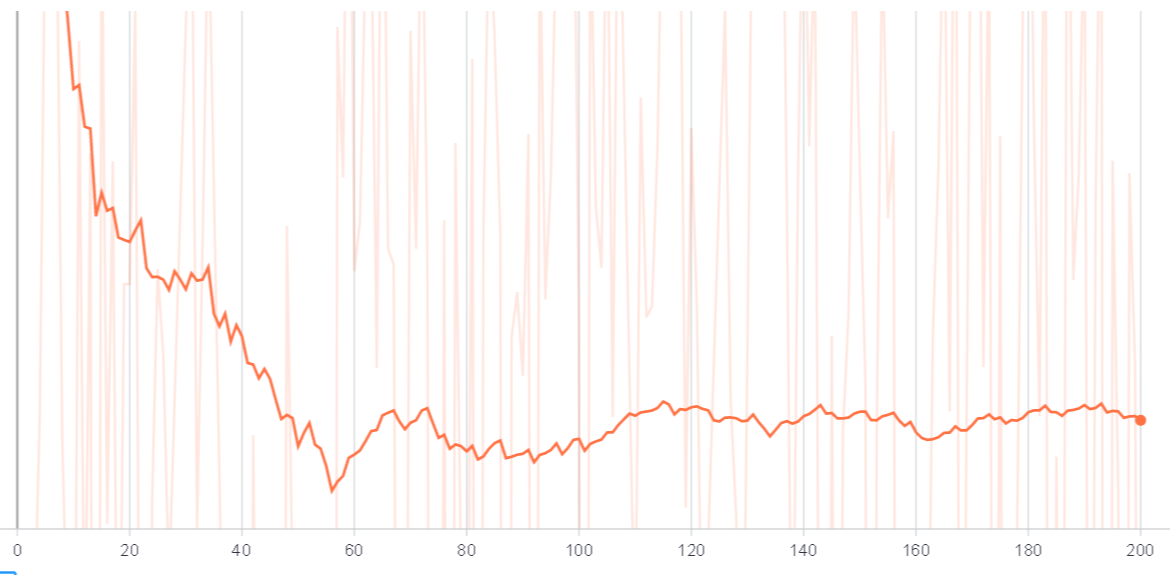
\includegraphics[width=0.5\textwidth]{loss.png}
\caption[width=0.5\textwidth]{Loss value decreasing in time as the model is learning}
\end{figure}

\section {Rest API}

We implemented the REST API with the help of the Flask microframework. The service was written in the same project as the model. This ensures a quick and reliable communication between the two. 
The server is configured to run on port 5000. Two routes were defined: \texttt{/drums} and \texttt{/vocals}. To receive the drums source, the client must make a Post request to \texttt{/drums} while providing the audio file to be processed under the name \texttt{file}. For receiving the vocals source a similar request is sent, but this time to the \texttt{/vocals} route.

 The server methods that are linked to the two available routes are almost identical. They receive the audio file, and verify the file is the correct format. If it passes the check, the files are read and transformed into waveforms. The Flask framework procures the methods that are used for verifying and saving the file.  From this point on, this waveform passes through all the processes needed in order to be given to the model as input. After the model predicts the two different sources, the source requested by the user is transformed back into an audio file and sent back to the client as the response to the POST request.

The structure of the service, as well as the flow of data is efficient and straight-forward. Different technologies could be used to create a REST API, but using Flask we managed to keep it in the same environment as the separation algorithm.

\section {Mobile Interface}

The mobile interface was done in Flutter. It has a very similar structure to the web application. The Flutter framework relies on \texttt{Widgets} to display objects. These \texttt{Widgets} have a lot of similarities to the \texttt{Components} from React like being capable of storing information in a State, and only rendering the components that have changed. 

The application has a single screen, that contains all the information and features we need. In the top of the screen is a file picker that lets us select the audio file. Information on this file is displayed making us certain that the correct file is loaded. Two command buttons are in the bottom half of the screen. Pressing each one will send the selected file to the server and wait for a response. If the server is working, the result audio file corresponding to our previous choice is received and saved to the mobile device. 

For connecting with the REST API, we designed a Server Helper. Inside it we take advantage of the http package available in Dart to simply make the post requests. The selected audio is sent by these requests. The response from the server will contain an audio file. This file will be saved on the device, and the user will be informed of this action. 

The application works on both Android and iOS. Slight differences can be seen when using the file picker. 

\begin{figure}[h]
\centering
\label {fig: mobile}
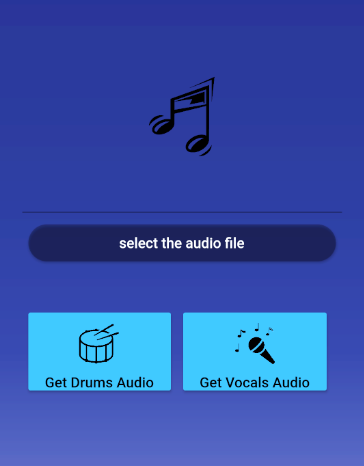
\includegraphics[width=0.5\textwidth]{mobilegui.png}
\caption[width=0.5\textwidth]{screenshot of the current mobile app design}
\end{figure}

\section {Web Interface}

For the web-based user interface, we used React. Although we could have created a simple web-page using HTML and CSS, using React and making a solid structure makes expanding and refactoring it a lot easier. This current website can be transformed into a complex web application using the same technologies and source code. 

Only the default route is currently accessible. Trying to go on any other route will give an \texttt{Error 404} Page. On this landing page we notice 3 buttons. The first one when pressed opens a file dialog that can select an audio file in \texttt{.wav} or \texttt{.mp3} format. This is the file that is send to the back-end. After selecting, pressing on one of the remaining two buttons will send a request tot the server. Pressing each one will send a POST request to the server, containing the selected audio file. The web application will wait for a response, which hopefully will contain the requested separated audio. The file will automatically download to the user’s machine. 
A multitude of HTML (HyperText Markup Language) Elements are used to define the structure of the webpage. The \texttt{Input} element inside a \texttt{Form} is used to select the audio file and two \texttt{Button} elements are used to call the functions that send the POST requests. Every element is styled with CSS (Cascading Style Sheets) in order to give them a pleasant look. 

\begin{figure}[h]
\centering
\label {fig: web}
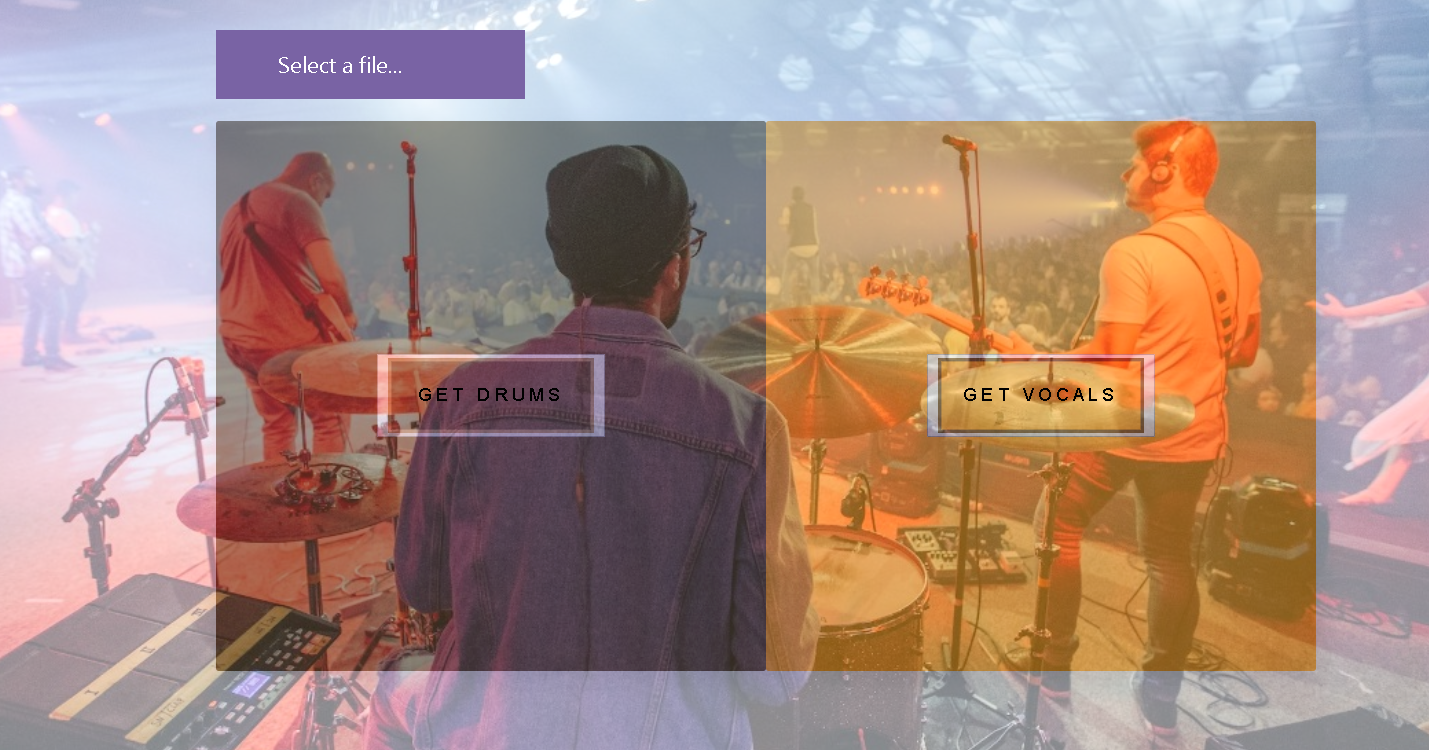
\includegraphics[width=0.5\textwidth]{webgui.png}
\caption[width=0.5\textwidth]{screenshot of the current web page design}
\end{figure}

\end{document}
